% ********** Rozdział 2 **********
\chapter{Opis struktury projektu}
Projekt został zbudowany w oparciu o modułową architekturę, dzięki której łatwo można zarządzać poszczególnymi częściami systemu. Główne komponenty to:
\begin{figure}[htbp]
  \centering
  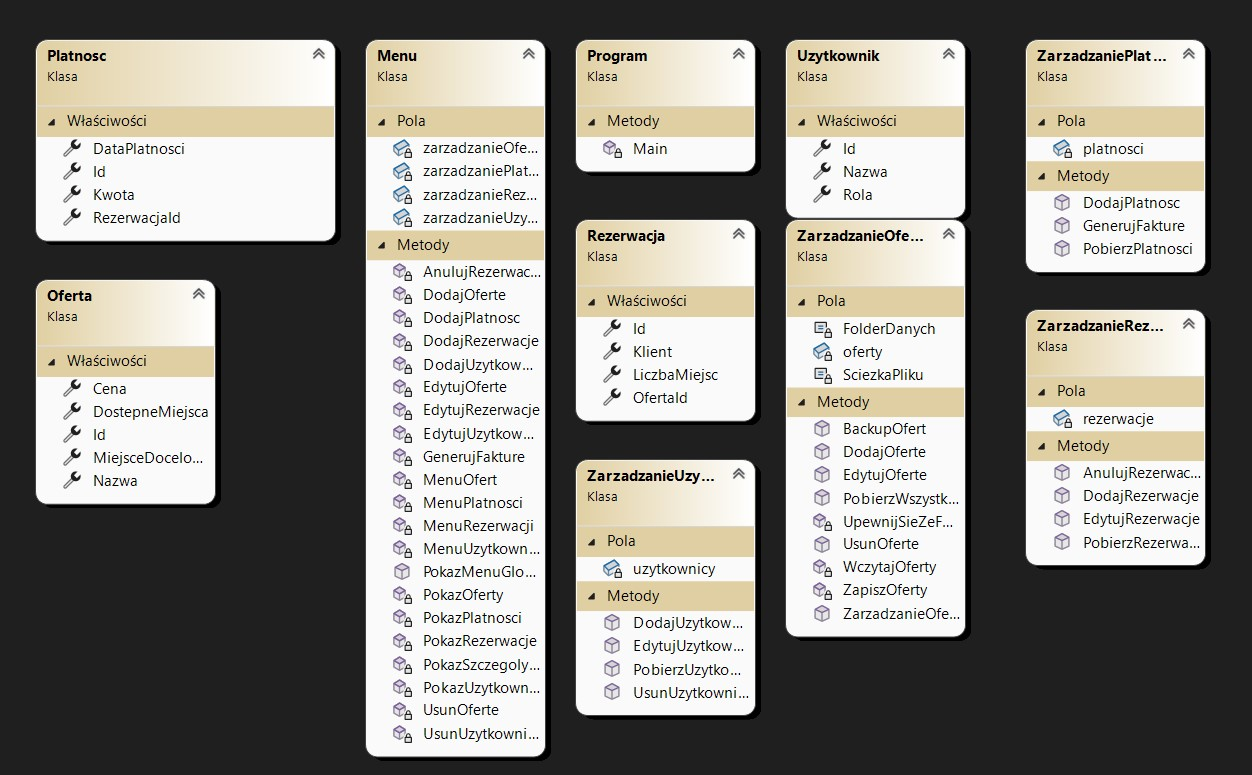
\includegraphics[width=1\textwidth]{figures/diagram_klas.jpg} 
  \caption{Diagram klas użytych w programie.}
  \label{fig:obrazek}
\end{figure}

\noindent \textbf{Modele Danych:}
\begin{itemize}
    \item \textbf{Oferta} – reprezentuje ofertę turystyczną, przechowując dane takie jak nazwa, destynacja, cena i dostępność miejsc.
    \item \textbf{Rezerwacja} – zawiera informacje o rezerwacjach, w tym identyfikator oferty, dane klienta oraz liczbę zarezerwowanych miejsc.
    \item \textbf{Płatność} – przechowuje dane dotyczące płatności, w tym kwotę, datę oraz powiązanie z konkretną rezerwacją.
    \item \textbf{Użytkownik} – model użytkownika systemu, który pozwala na zarządzanie kontami i uprawnieniami.
\end{itemize}
\noindent \textbf{Logika Biznesowa:}
Każdy z modułów zarządzających (oferty, rezerwacje, płatności, użytkownicy) zawiera operacje CRUD, czyli funkcje umożliwiające tworzenie, odczyt, modyfikację i usuwanie danych. Moduły te korzystają z wbudowanych bibliotek .NET, takich jak \texttt{System.IO} i \texttt{System.Text.Json}, do operacji na plikach oraz serializacji danych.

\noindent \textbf{Warstwa Prezentacji:}
Interfejs użytkownika opiera się na prostym menu konsolowym, które umożliwia nawigację między poszczególnymi modułami systemu. Użytkownik może wybrać odpowiednią opcję, aby wykonać operacje związane z zarządzaniem ofertami, rezerwacjami, płatnościami i kontami.

\noindent \textbf{Punkt Wejścia:}
Program rozpoczyna działanie od metody \texttt{Main()}, która inicjuje obiekt odpowiedzialny za wyświetlenie menu głównego.



\section{Modele Danych}
\subsection*{Klasa \textbf{Oferta}}
\begin{itemize}
    \item \textbf{Atrybuty:}
    \begin{itemize}
        \item \texttt{int Id} -- unikalny identyfikator oferty.
        \item \texttt{string Nazwa} -- nazwa oferty (np. "Wakacje w Grecji").
        \item \texttt{string MiejsceDocelowe} -- miejsce docelowe oferty.
        \item \texttt{decimal Cena} -- cena oferty; typ \texttt{decimal} zapewnia dokładność operacji finansowych.
        \item \texttt{int DostepneMiejsca} -- liczba dostępnych miejsc w ofercie.
    \end{itemize}
    \item \textbf{Metody:}  
    Klasa wykorzystuje autogenerowane właściwości (get; set;), pełniąc funkcję przechowywania danych bez dodatkowej logiki.
\end{itemize}

\subsection*{Klasa \textbf{Rezerwacja}}
\begin{itemize}
    \item \textbf{Atrybuty:}
    \begin{itemize}
        \item \texttt{int Id} -- unikalny identyfikator rezerwacji.
        \item \texttt{int OfertaId} -- identyfikator powiązanej oferty.
        \item \texttt{string Klient} -- dane klienta (np. imię i nazwisko) dokonującego rezerwacji.
        \item \texttt{int LiczbaMiejsc} -- liczba miejsc zarezerwowanych przez klienta.
    \end{itemize}
    \item \textbf{Metody:}  
    Podobnie jak w klasie \textbf{Oferta}, właściwości przechowują dane bez dodatkowej logiki.
\end{itemize}

\subsection*{Klasa \textbf{Platnosc}}
\begin{itemize}
    \item \textbf{Atrybuty:}
    \begin{itemize}
        \item \texttt{int Id} -- unikalny identyfikator płatności.
        \item \texttt{int RezerwacjaId} -- identyfikator rezerwacji, do której odnosi się płatność.
        \item \texttt{decimal Kwota} -- kwota płatności.
        \item \texttt{string DataPlatnosci} -- data dokonania płatności (jako ciąg znaków).
    \end{itemize}
    \item \textbf{Metody:}  
    Klasa służy do przechowywania danych dotyczących płatności przy użyciu autogenerowanych właściwości.
\end{itemize}

\subsection*{Klasa \textbf{Uzytkownik}}
\begin{itemize}
    \item \textbf{Atrybuty:}
    \begin{itemize}
        \item \texttt{int Id} -- unikalny identyfikator użytkownika.
        \item \texttt{string Nazwa} -- nazwa lub login użytkownika.
        \item \texttt{string Rola} -- rola przypisana użytkownikowi (np. administrator, pracownik, klient).
    \end{itemize}
    \item \textbf{Metody:}  
    Podstawową funkcją klasy jest przechowywanie informacji o użytkowniku.
\end{itemize}

\section{Klasy Zarządzające (Service/Manager Classes)}
\subsection*{Klasa \textbf{ZarzadzanieOfertami}}
\begin{itemize}
    \item \textbf{Atrybuty:}
    \begin{itemize}
        \item \texttt{const string FolderDanych} -- nazwa folderu (np. "Dane") do przechowywania pliku.
        \item \texttt{const string SciezkaPliku} -- pełna ścieżka do pliku JSON (np. "Dane/oferty.json").
        \item \texttt{List<Oferta> oferty} -- lista ofert wczytanych z pliku.
    \end{itemize}
    \item \textbf{Kluczowe Metody:}
    \begin{itemize}
        \item \texttt{ZarzadzanieOfertami()} -- Konstruktor; sprawdza istnienie folderu (metoda \texttt{UpewnijSieZeFolderIstnieje()}), tworzy plik JSON, jeżeli nie istnieje, oraz wczytuje oferty (metoda \texttt{WczytajOferty()}).
        \item \texttt{UpewnijSieZeFolderIstnieje()} -- Sprawdza, czy folder \texttt{FolderDanych} istnieje; w razie potrzeby tworzy go.
        \item \texttt{WczytajOferty()} -- Odczytuje zawartość pliku JSON, deserializuje dane do listy obiektów \texttt{Oferta} i zwraca tę listę.
        \item \texttt{ZapiszOferty()} -- Serializuje listę ofert do formatu JSON i zapisuje ją w pliku.
        \item \texttt{PobierzWszystkieOferty()} -- Zwraca listę wszystkich ofert.
        \item \texttt{DodajOferte(Oferta oferta)} -- Przed dodaniem nowej oferty przypisuje jej unikalne \texttt{Id} i zapisuje ofertę.
        \item \texttt{EdytujOferte(int id, Oferta nowaOferta)} -- Wyszukuje ofertę po \texttt{Id} i aktualizuje jej dane (Nazwa, MiejsceDocelowe, Cena, DostepneMiejsca), a następnie zapisuje zmiany.
        \item \texttt{UsunOferte(int id)} -- Usuwa ofertę o podanym \texttt{Id} z listy i zapisuje zmiany.
        \item \texttt{BackupOfert()} -- Tworzy kopię zapasową pliku JSON z ofertami.
    \end{itemize}
\end{itemize}

\subsection*{Klasa \textbf{ZarzadzanieRezerwacjami}}
\begin{itemize}
    \item \textbf{Atrybuty:}
    \begin{itemize}
        \item \texttt{List<Rezerwacja> rezerwacje} -- lista rezerwacji przechowywana w pamięci.
    \end{itemize}
    \item \textbf{Kluczowe Metody:}
    \begin{itemize}
        \item \texttt{DodajRezerwacje(Rezerwacja rezerwacja)} -- Dodaje nową rezerwację, przypisując jej unikalne \texttt{Id}.
        \item \texttt{EdytujRezerwacje(int id, Rezerwacja nowaRezerwacja)} -- Wyszukuje rezerwację po \texttt{Id} i aktualizuje jej dane (OfertaId, Klient, LiczbaMiejsc).
        \item \texttt{AnulujRezerwacje(int id)} -- Usuwa rezerwację o określonym \texttt{Id} z listy.
        \item \texttt{PobierzRezerwacje()} -- Zwraca aktualną listę rezerwacji.
    \end{itemize}
\end{itemize}

\subsection*{Klasa \textbf{ZarzadzaniePlatnosciami}}
\begin{itemize}
    \item \textbf{Atrybuty:}
    \begin{itemize}
        \item \texttt{List<Platnosc> platnosci} -- lista płatności.
    \end{itemize}
    \item \textbf{Kluczowe Metody:}
    \begin{itemize}
        \item \texttt{DodajPlatnosc(Platnosc platnosc)} -- Dodaje nową płatność, przypisując jej unikalne \texttt{Id}.
        \item \texttt{PobierzPlatnosci()} -- Zwraca listę wszystkich płatności.
        \item \texttt{GenerujFakture(int platnoscId)} -- Wyszukuje płatność po \texttt{Id} i zwraca sformatowaną fakturę zawierającą dane płatności; w przypadku braku płatności, zwraca komunikat o błędzie.
    \end{itemize}
\end{itemize}

\subsection*{Klasa \textbf{ZarzadzanieUzytkownikami}}
\begin{itemize}
    \item \textbf{Atrybuty:}
    \begin{itemize}
        \item \texttt{List<Uzytkownik> uzytkownicy} -- lista użytkowników.
    \end{itemize}
    \item \textbf{Kluczowe Metody:}
    \begin{itemize}
        \item \texttt{DodajUzytkownika(Uzytkownik uzytkownik)} -- Dodaje nowego użytkownika, nadając mu unikalne \texttt{Id}.
        \item \texttt{EdytujUzytkownika(int id, Uzytkownik nowyUzytkownik)} -- Znajduje użytkownika o danym \texttt{Id} i aktualizuje jego dane (Nazwa, Rola).
        \item \texttt{UsunUzytkownika(int id)} -- Usuwa użytkownika o podanym \texttt{Id} z listy.
        \item \texttt{PobierzUzytkownikow()} -- Zwraca listę wszystkich użytkowników.
    \end{itemize}
\end{itemize}

\section{Warstwa Interfejsu Użytkownika}
\subsection*{Klasa \textbf{Menu}}
\begin{itemize}
    \item \textbf{Atrybuty:}
    \begin{itemize}
        \item \texttt{ZarzadzanieOfertami zarzadzanieOfertami} -- obiekt do zarządzania ofertami.
        \item \texttt{ZarzadzanieRezerwacjami zarzadzanieRezerwacjami} -- obiekt do zarządzania rezerwacjami.
        \item \texttt{ZarzadzaniePlatnosciami zarzadzaniePlatnosciami} -- obiekt do obsługi płatności.
        \item \texttt{ZarzadzanieUzytkownikami zarzadzanieUzytkownikami} -- obiekt do zarządzania użytkownikami.
    \end{itemize}
    \item \textbf{Kluczowe Metody:}
    \begin{itemize}
        \item \texttt{PokazMenuGlowne()} -- Uruchamia główną pętlę interakcji, wyświetlając menu główne i kierując użytkownika do odpowiednich podmenu.
        \item \textbf{Podmenu ofert:}
        \begin{itemize}
            \item \texttt{MenuOfert()} -- Wyświetla opcje zarządzania ofertami.
            \item \texttt{PokazOferty()} -- Prezentuje listę wszystkich ofert.
            \item \texttt{PokazSzczegolyOferty()} -- Po podaniu ID, wyświetla szczegóły wybranej oferty.
            \item \texttt{DodajOferte()} -- Pobiera dane od użytkownika, tworzy nową ofertę i wywołuje metodę dodawania w module ofert.
            \item \texttt{EdytujOferte()} -- Umożliwia edycję istniejącej oferty.
            \item \texttt{UsunOferte()} -- Umożliwia usunięcie oferty.
        \end{itemize}
        \item \textbf{Podmenu rezerwacji:}
        \begin{itemize}
            \item \texttt{MenuRezerwacji()} -- Wyświetla opcje związane z rezerwacjami.
            \item \texttt{DodajRezerwacje()} -- Pobiera dane wejściowe i dodaje nową rezerwację.
            \item \texttt{EdytujRezerwacje()} -- Umożliwia edycję wybranej rezerwacji.
            \item \texttt{AnulujRezerwacje()} -- Pozwala na anulowanie rezerwacji.
            \item \texttt{PokazRezerwacje()} -- Wyświetla listę rezerwacji.
        \end{itemize}
        \item \textbf{Podmenu płatności:}
        \begin{itemize}
            \item \texttt{MenuPlatnosci()} -- Wyświetla opcje związane z płatnościami.
            \item \texttt{DodajPlatnosc()} -- Dodaje nową płatność na podstawie danych wejściowych.
            \item \texttt{PokazPlatnosci()} -- Prezentuje listę płatności.
            \item \texttt{GenerujFakture()} -- Generuje i wyświetla fakturę dla wybranej płatności.
        \end{itemize}
        \item \textbf{Podmenu użytkowników:}
        \begin{itemize}
            \item \texttt{MenuUzytkownikow()} -- Wyświetla opcje zarządzania użytkownikami.
            \item \texttt{DodajUzytkownika()} -- Dodaje nowego użytkownika.
            \item \texttt{EdytujUzytkownika()} -- Umożliwia edycję danych użytkownika.
            \item \texttt{UsunUzytkownika()} -- Pozwala na usunięcie użytkownika.
            \item \texttt{PokazUzytkownikow()} -- Wyświetla listę użytkowników.
        \end{itemize}
    \end{itemize}
\end{itemize}

\section{Klasa Główna}
\subsection*{Klasa \textbf{Program}}
\begin{itemize}
    \item \textbf{Metody:}
    \begin{itemize}
        \item \texttt{Main()} -- Główna metoda wejścia do aplikacji. Tworzy instancję klasy \textbf{Menu} i wywołuje metodę \texttt{PokazMenuGlowne()}, inicjując interakcję z użytkownikiem.
    \end{itemize}
\end{itemize}

Hierarchia klas w systemie zarządzania biurem podróży została zaprojektowana w sposób modularny, co umożliwia oddzielenie modelu danych (Oferta, Rezerwacja, Platnosc, Uzytkownik) od logiki biznesowej (moduły ZarzadzanieOfertami, ZarzadzanieRezerwacjami, ZarzadzaniePlatnosciami, ZarzadzanieUzytkownikami) oraz interfejsu użytkownika (klasa Menu). Kluczowe metody umożliwiają wykonywanie operacji CRUD na danych oraz zapewniają prostą obsługę aplikacji przez użytkownika. Główny punkt wejścia, metoda Main() w klasie Program, inicjuje cały proces, uruchamiając główne menu i umożliwiając interakcję z systemem.

% ********** Koniec rozdziału **********
